\documentclass[12pt]{article}
\usepackage[english]{babel}
\usepackage[T1]{fontenc}
\usepackage{color}
\usepackage{fancyvrb}
\usepackage{hyperref}
\usepackage[procnames]{listings}
\usepackage{blindtext}
\usepackage{graphicx}
\usepackage{float}

\begin{document}

\begin{titlepage}
	
\title{\vspace{60mm}Reducing noise in protein multialignments}
\subparagraph{\url{https://github.com/msarrias/protein_multial_noise_reduction}}
\author{Marina Herrera Sarrias}
\date{January 6, 2019}


\clearpage\maketitle
\thispagestyle{empty}
\end{titlepage}
\pagenumbering{roman}


\section*{Abstract}

In this research a noise-reduction method is implemented in protein multialigments to evaluate its impact on phylogenic inference. The data used in this project is a reduced data set from the  original data used by the creators of \href{http://trimal.cgenomics.org}{TrimAI}. To test the data the program \href{http://fastphylo.sourceforge.net/}{fastprot} was used to obtain the distance matrices and \href{http://fastphylo.sourceforge.net/}{fnj} to infer a phylogenic tree for each alignment.\href{https://dendropy.org/}{Dendropy} has been used to measure the symmetric distance between the inferred tree and the reference tree. The results obtained show that although in most of the cases the effect of reducing the noise from the alignments was ineffective, when it was it had a reducing effect on the distance, with a greater effect on symmetric alingments with greater average amount of mutations per site.  This study focuses in determining whether the noise reduction makes any effect in the symmetric distance calculation. 

\addcontentsline{toc}{section}{Abstract}
\clearpage
	
\tableofcontents
\clearpage

\pagenumbering{arabic}
\section{Introduction}

The implemented noise-reduction method evaluates a multialigment column as noisy if there are more than $50\%$ indels, at least $50\%$ of the amino acids are unique and non of the amino acids appear more than twice. Each column takes the form of a sequence of amino acids given a position of the aligned sequences.

The reduced data set used in this project is composed by six different sub-directories, each sub-directory contains a reference tree and 300 alignments created by evolving sequences along the reference tree. Each pair of sub-directories present an average amount of mutations of 0.5, 1.0 and 2.0 per sequence site. Also, per each mutation rate there is one symmetric reference tree and one asymmetric reference tree.

For validating the effect of reducing reducing 

\section{Results and Discussion}\\

After verifying the correctness of the program and processing the six data sets  Table \ref{table:freqtable} is the resulting frequency table of the six possible symmetric distance scenarios.\\

In most of the cases the original tree and the noise reduced  alignment tree are the same, this means that the method applied did not have any effect in most of the alignments, although the cases in which the effect is not the same between the original and noise reduced inferred tree, the effect of reducing noise in the alignments makes the new noise reduced data to have a smaller symmetric distance with the reference tree, while there are fewer cases in which the effect is the opposite.\\

The reference tree is recovered with a greater frequency when the tree is symmetric and the average amount of mutations per sequence site is smaller, meaning that the symmetric difference is equal to 0. According to the frequency values the reference tree was recovered 3 times by the noise reduced tree  while it was recovered 5 times by the original multialignment inferred tree. 

Table \ref{table:statistics} gives statistical information about the six data sets. In most of the cases, both inferred trees take the same values, except  for the means of the noise reduced inferred trees symmetric difference which is slightly smaller and the maximum noise reduced inferred tree of the Asymmetric 2.0 sub-directory. Although both frequency values are mostly the same on all of the original and noise reduced cases, the values tend to be smaller for the symmetric sets than for the asymmetric sets, the values tend to  increment as the average amount of mutations increments as well.


\begin{table}[H]
	\small\addtolength{\tabcolsep}{-5pt}
	\begin{tabular}{l|c|c|c|c|c|c|l}
		\cline{2-7}
		\textbf{} & \multicolumn{1}{l|}{Asymm\_0.5} & \multicolumn{1}{l|}{Asymm\_1.0} & \multicolumn{1}{l|}{Asymm\_ 2.0} & \multicolumn{1}{l|}{Symm\_0.5} & \multicolumn{1}{l|}{Symm\_1.0} & \multicolumn{1}{l|}{Symm\_2.0} &  \\ \cline{1-7}
		\multicolumn{1}{|l|}{Original \textgreater Reduced} & 45 & 60 & 79 & 44 & 59 & 83 &  \\ \cline{1-7}
		\multicolumn{1}{|l|}{Original \textless Reduced} & 48 & 54 & 45 & 28 & 36 & 54 &  \\ \cline{1-7}
		\multicolumn{1}{|l|}{Original = Reduced} & 206 & 186 & 176 & 214 & 201 & 162 &  \\ \cline{1-7}
		\multicolumn{1}{|l|}{Original = 0} & 0 & 0 & 0 & 4 & 1 & 0 &  \\ \cline{1-7}
		\multicolumn{1}{|l|}{Reduced = 0} & 0 & 0 & 0 & 2 & 1 & 0 &  \\ \cline{1-7}
		\multicolumn{1}{|l|}{Original \& Red = 0} & 1 & 0 & 0 & 8 & 2 & 1 &  \\ \cline{1-7}
		\multicolumn{1}{|l|}{\textbf{Total}} & 300 & 300 & 300 & 300 & 300 & 300 &  \\ \cline{1-7}
	\end{tabular}
\caption{Data sets frequencies referring to the symmetric distance of the original and reduced newick trees with the reference tree.}
\label{table:freqtable}
\end{table}

\begin{table}[H]
	\small\addtolength{\tabcolsep}{-5pt}
	\begin{tabular}{lcccccccc}
		\cline{2-9}
		\multicolumn{1}{c|}{\textbf{}} & \multicolumn{2}{c|}{Minimum} & \multicolumn{2}{c|}{Maximum} & \multicolumn{2}{c|}{Mean} & \multicolumn{2}{c|}{Median} \\ \cline{2-9} 
		\multicolumn{1}{l|}{\textbf{}} & \multicolumn{1}{l|}{Original} & \multicolumn{1}{l|}{Reduced} & \multicolumn{1}{l|}{Original} & \multicolumn{1}{l|}{Reduced} & \multicolumn{1}{l|}{Original} & \multicolumn{1}{l|}{Reduced} & \multicolumn{1}{l|}{Original} & \multicolumn{1}{l|}{Reduced} \\ \hline
		\multicolumn{1}{|l|}{Asymmetric 0.5} & \multicolumn{1}{c|}{2} & \multicolumn{1}{c|}{2} & \multicolumn{1}{c|}{18} & \multicolumn{1}{c|}{18} & \multicolumn{1}{c|}{7.63} & \multicolumn{1}{c|}{7.62} & \multicolumn{1}{c|}{8} & \multicolumn{1}{c|}{8} \\ \hline
		\multicolumn{1}{|l|}{Asymmetric 1.0} & \multicolumn{1}{c|}{2} & \multicolumn{1}{c|}{2} & \multicolumn{1}{c|}{18} & \multicolumn{1}{c|}{18} & \multicolumn{1}{c|}{9.43} & \multicolumn{1}{c|}{9.39} & \multicolumn{1}{c|}{10} & \multicolumn{1}{c|}{10} \\ \hline
		\multicolumn{1}{|l|}{Asymmetric 2.0} & \multicolumn{1}{c|}{4} & \multicolumn{1}{c|}{4} & \multicolumn{1}{c|}{22} & \multicolumn{1}{c|}{20} & \multicolumn{1}{c|}{12.34} & \multicolumn{1}{c|}{11.99} & \multicolumn{1}{c|}{12} & \multicolumn{1}{c|}{12} \\ \hline
		\multicolumn{1}{|l|}{Symmetric 0.5} & \multicolumn{1}{c|}{2} & \multicolumn{1}{c|}{2} & \multicolumn{1}{c|}{10} & \multicolumn{1}{c|}{10} & \multicolumn{1}{c|}{4.66} & \multicolumn{1}{c|}{4.55} & \multicolumn{1}{c|}{4} & \multicolumn{1}{c|}{4} \\ \hline
		\multicolumn{1}{|l|}{Symmetric 1.0} & \multicolumn{1}{c|}{2} & \multicolumn{1}{c|}{2} & \multicolumn{1}{c|}{12} & \multicolumn{1}{c|}{12} & \multicolumn{1}{c|}{6.23} & \multicolumn{1}{c|}{6.05} & \multicolumn{1}{c|}{6} & \multicolumn{1}{c|}{6} \\ \hline
		\multicolumn{1}{|l|}{Symmetric 2.0} & \multicolumn{1}{c|}{2} & \multicolumn{1}{c|}{2} & \multicolumn{1}{c|}{16} & \multicolumn{1}{c|}{16} & \multicolumn{1}{c|}{8.91} & \multicolumn{1}{c|}{8.65} & \multicolumn{1}{c|}{8} & \multicolumn{1}{c|}{8} \\ \hline
		& \multicolumn{1}{l}{} & \multicolumn{1}{l}{} & \multicolumn{1}{l}{} & \multicolumn{1}{l}{} & \multicolumn{1}{l}{} & \multicolumn{1}{l}{} & \multicolumn{1}{l}{} & \multicolumn{1}{l}{}
	\end{tabular}
	\caption{Data sets statistics referring to the symmetric distance of the original and reduced newick trees with the reference tree.}
	\label{table:statistics}
\end{table}

Referring to Figure \ref{table:averg} the noise reduction performance was slightly higher on the symmetric sets than in the asymmetric, the noise reduction average also tends to grow as the average amount of mutations increments as well.



\begin{table}[H]
	\centering
	\small\addtolength{\tabcolsep}{-5pt}
	\begin{tabular}{l|c|l}
		\cline{2-2}
		\textbf{} & \multicolumn{1}{l|}{Average Noise Reduction} &  \\ \cline{1-2}
		\multicolumn{1}{|l|}{Asymmetric 0.5} & 0.146 &  \\ \cline{1-2}
		\multicolumn{1}{|l|}{Asymmetric 1.0} & 0.199 &  \\ \cline{1-2}
		\multicolumn{1}{|l|}{Asymmetric 2.0} & 0.252 &  \\ \cline{1-2}
		\multicolumn{1}{|l|}{Symmetric 0.5} & 0.172 &  \\ \cline{1-2}
		\multicolumn{1}{|l|}{Symmetric 1.0} & 0.221 &  \\ \cline{1-2}
		\multicolumn{1}{|l|}{Symmetric 2.0} & 0.282 &  \\ \cline{1-2}
	\end{tabular}
\caption{Average noise reduction performed per data set}
\label{table:averg}
\end{table}


\section{Methods and Materials}
The project was developed  working in three different major tasks separately which were later joint together to consolidate the program and reproduce the exploratory data analysis. The main objective for creating three different scripts, for each functionality was to initially test the data and the control cases, before unifying them all in a single script and running the program on the fixed data set.\\

A \href{https://github.com/msarrias/protein_multial_noise_reduction}{Github repository} was created in order to version control the program. The Laboratory notebook contains all details regarding the projects evolution, it was created using a Jupyter notebook Markdown and later compiled into a HTML file. It can be found on the \href{https://github.com/msarrias/protein_multial_noise_reduction/tree/master/results}{Github repository} \\

Following the \href{https://journals.plos.org/ploscompbiol/article?id=10.1371/journal.pcbi.1000424#s6}{course centerpiece guideline}, controls were introduced along the project as well error handling. When an error occurs the program aborts and prints a message to standard error. All standard-in files are read by robust libraries. 
%The program do not creates a temporary name for the output file.%
A sub-directory containing a subset of the fixed data set was created in order to test the program, controls for different scenarios were also introduced to ensure the program functionality. No input is required for testing the data, either for running the main program.\\

\subsection{Running: run\_program.py}

run\_program.py performs all the project's required tasks in different stages:

\begin{enumerate}
	\item Reduce protein multialignment noise: 
The program will firstly takes an alignment from standard-in, filter the columns and write a new file containing the noise reduced multi-alignment. 
In order to illustrate the functionality of the program,   \href{http://doua.prabi.fr/software/seaview}{Seaview} was used as a graphical interface for the following example.\\

 Figure \ref{fig:al_1} shows the original alignment for the s001.align.1.msl file, corresponding to the asymmetric\_0.5 subdirectory. Figure \ref{fig:al_2} shows the alignment after the noise reduction was performed. In this particular case the reduced noise  represented a $17.08\%$ of the original sequence.

\begin{figure}[H]
	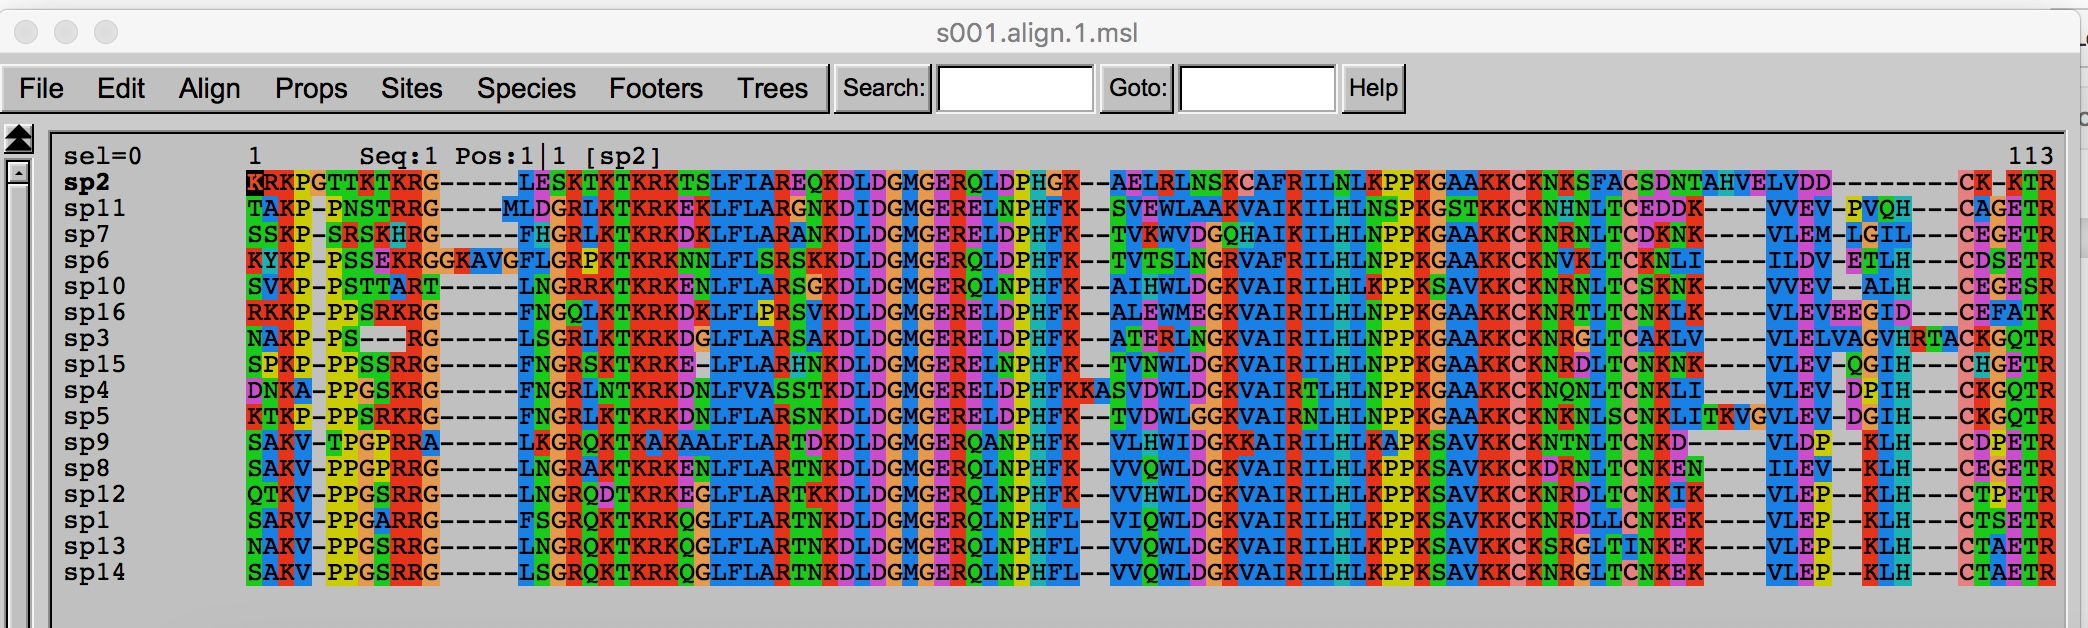
\includegraphics[width=\linewidth]{labnotes2.png}
	\caption{Original s001.align.1.msl}
	\label{fig:al_1}
\end{figure}

\begin{figure}[H]
	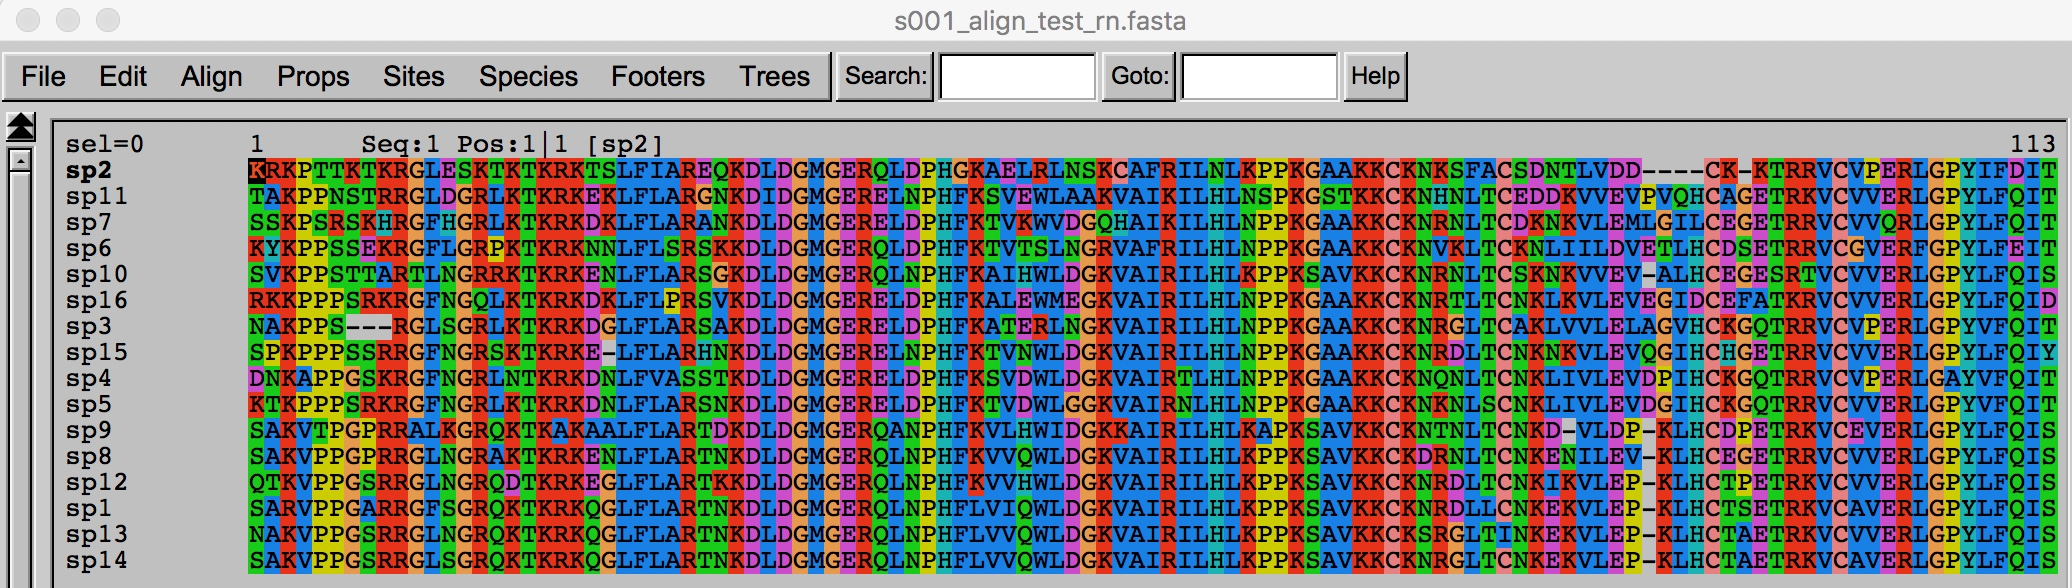
\includegraphics[width=\linewidth]{labnotes_1.png}
	\caption{s001.align.1.msl after noise reduction}
	\label{fig:al_2}
\end{figure}
	
	\item Generate phylogenetic trees:
 On the second stage, the program will pars through all the alignments available in the data directory (original and noise reduced), and using the  \href{http://fastphylo.sourceforge.net/}{fastphylo} programs (fastprot and fnj) will compute a distance matrix and generate a phylogenetic tree per alignment. In order to accomplish this task the program uses a sub-process to pipe the matrix creation and generate the tree. As the symmetric distance (computed in next stage) only requires the tree's topology it will not be necessary to compute the branch length information.  \\
 
  Following the s001.align.1.msl alignment example both, the noise reduced and original alignment have the same phylogenetic tree shown in Figure \ref{fig:reducedoriginaltree} while the reference tree is represented by  Figure \ref{fig:referencetree}.
  
\begin{figure}[H]
	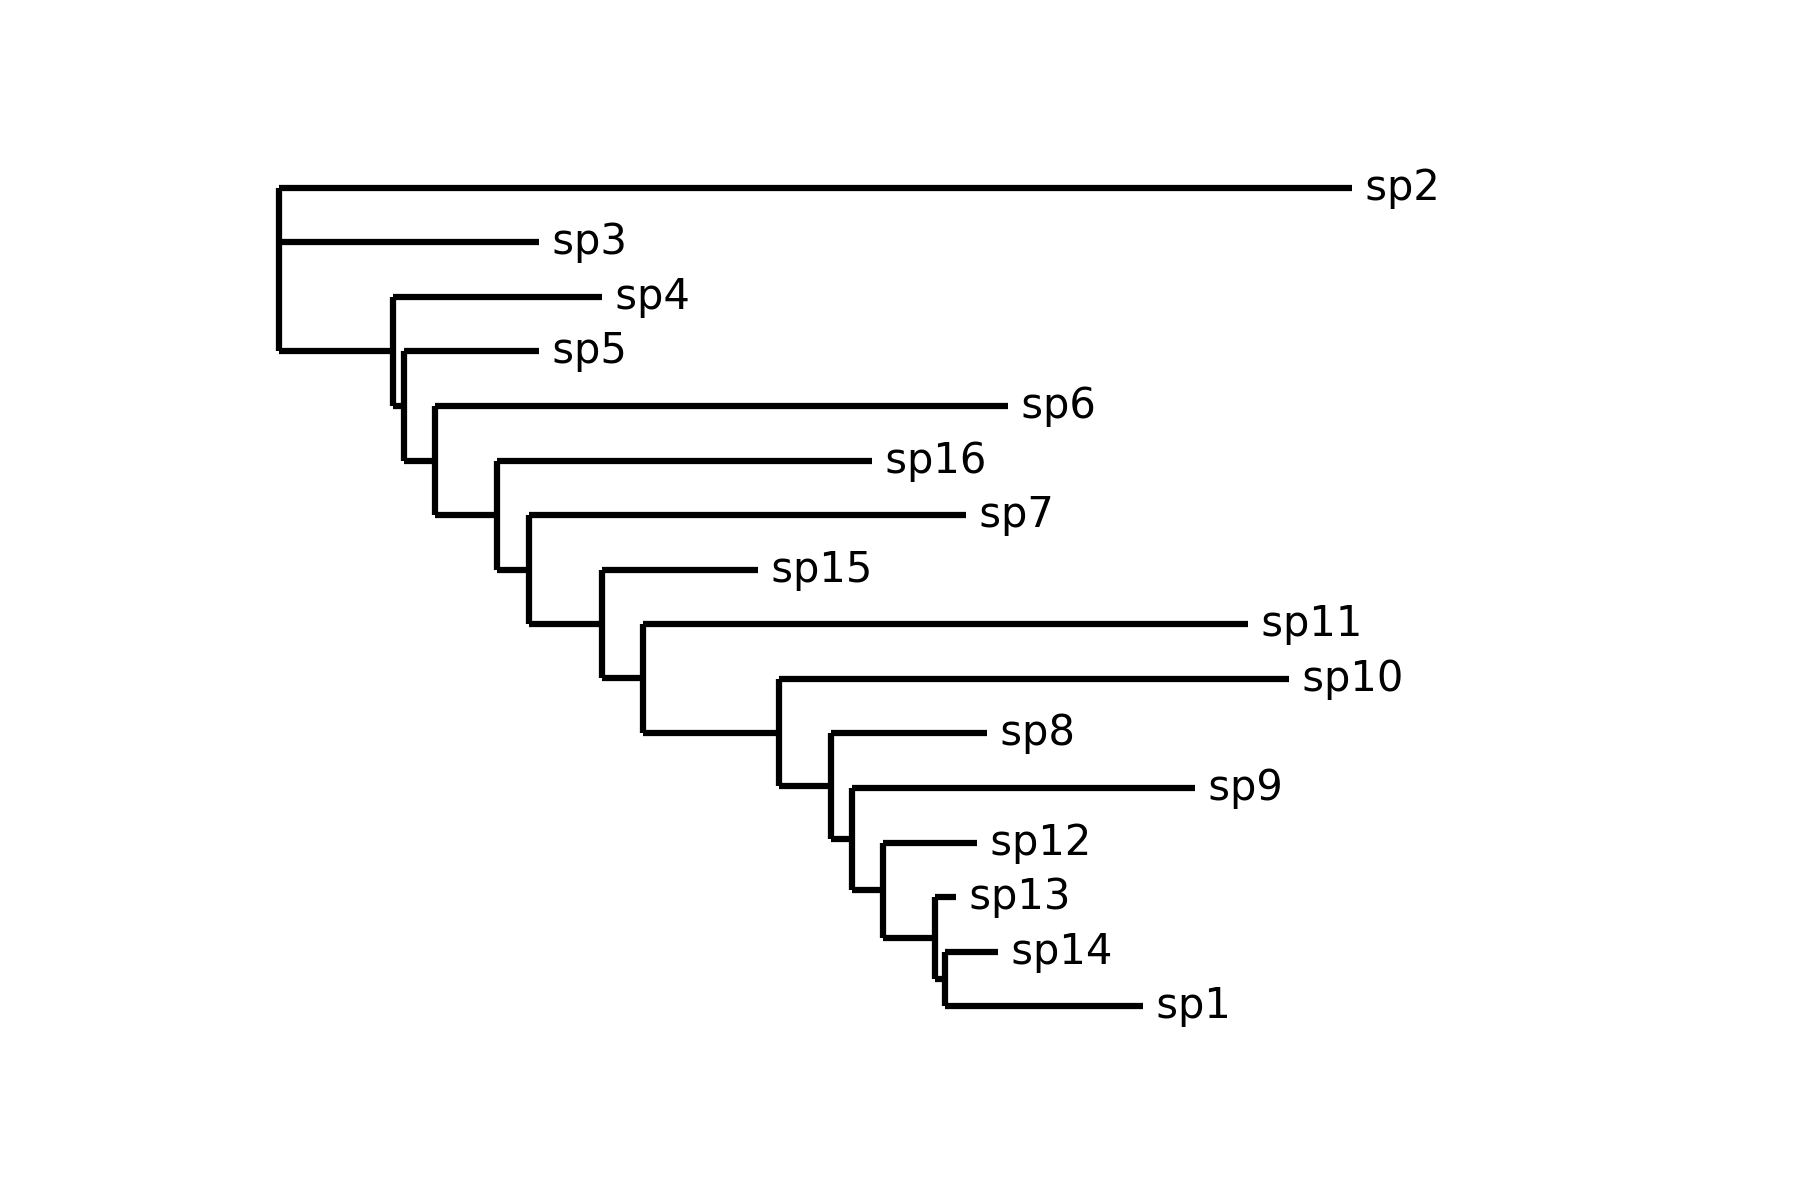
\includegraphics[width=.9\linewidth]{reference.png}
	\caption{asymmetric\_0.5.tree reference tree}
	\label{fig:referencetree}
\end{figure}

\begin{figure}[H]
	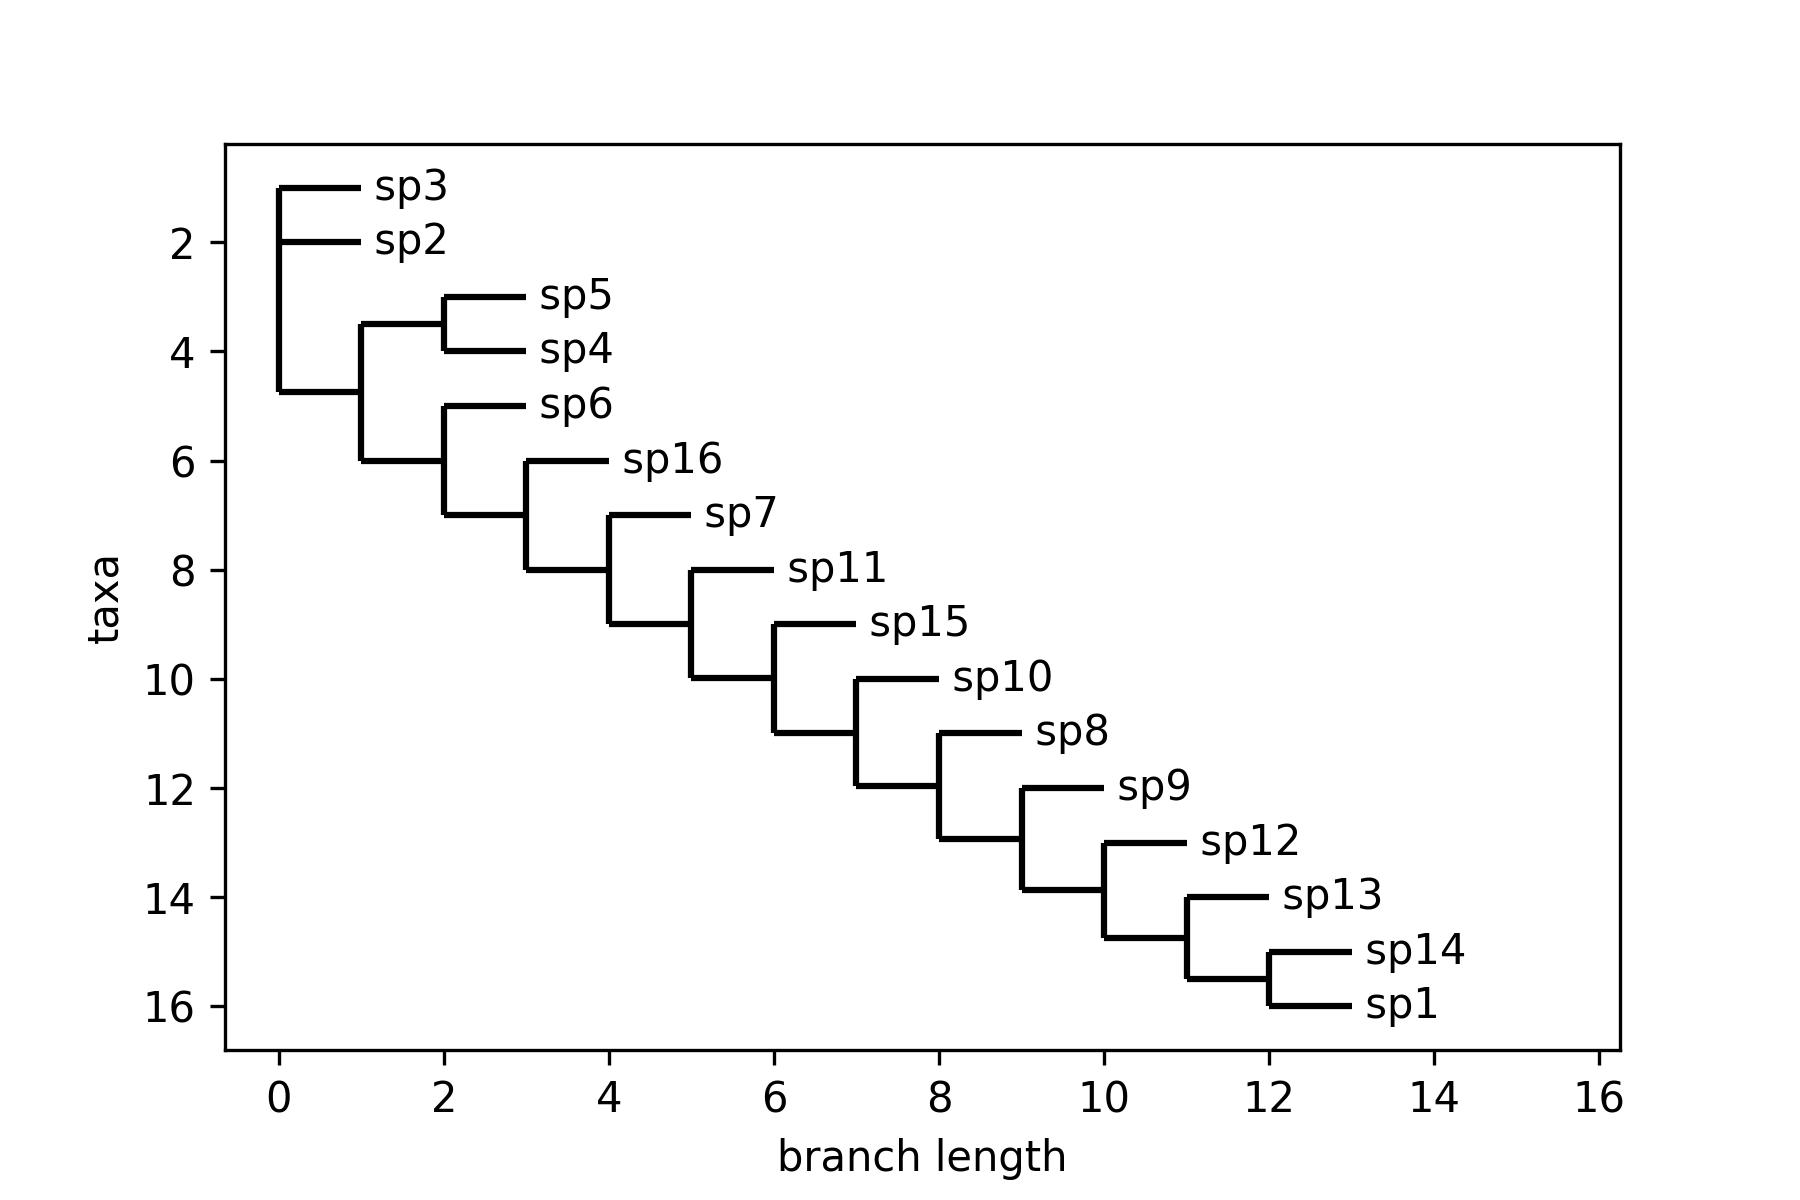
\includegraphics[width=.9\linewidth]{reduced_original.png}
	\caption{s001.align.1.msl original and noise reduced tree}
	\label{fig:reducedoriginaltree}
\end{figure}

\item Compute trees distances: At the final stage the program will compute the symmetric distance between the reference tree and the original and noise reduced tree using \href{https://dendropy.org/}{Dendropy}. The symmetric distance is a count of how many partitions there are among the two trees, that are on one tree and not on the other. Following the s001.align.1.msl, alignment example, as the original tree and noise reduced tree are the same the distance with the reference tree will be therefore the same, in this care 4.  
\end{enumerate}

\subsection{run\_program.py: Error handling and Control cases }

run\_program.py will abort if any of the following cases occur if:
\begin{itemize}
	\item There is an input introduction when executing the program.
	\item The data directory is empty.
	\item The data sub-directories are empty. (e.g asymmetric\_0.5).
	\item Any of the standard-in file (.msl,.tree) is empty.
	\item All the columns in the alignment are noisy. 
\end{itemize}
The program will  print a warning message but will not abort processing if:
\begin{itemize}
	\item The alignment do not have noisy columns.
	\item The noise reduction rate is greater than 0.5 times the original alignment.
\end{itemize}

All of the control files used for testing the accuracy of the script can be found in the  \href{https://github.com/msarrias/protein_multial_noise_reduction/tree/master/results/control_case_data}{Github repository}, results directory. Where a file for each case exposed before can be found.


\end{document}
